\startchapter{Real-time Cutting}
\label{chapter:Cutting}
One of the main objectives of virtual reality based surgical simulation systems is the removal of pathologic tissue 
\cite{Steinemann, Nienhuys2001a}. Cutting imposes many challenges in the development of a robust, interactive surgery 
simulation, not only because of the nonlinear geometric and material behavior exhibited by soft tissue but also due to the
complexity of introducing the cutting-induced discontinuity. In most publications, the progressive surgical cutting is modelled
by conventional finite element (FE) method, in which the high computational cost and error accumulation due to remeshing constrain 
the computational efficiency and accuracy. 

We developed our new cutting approach in the context of brain biopsy simulation. When an abnormality of the brain is suspected, 
Stereotactic (probing in three dimensions) brain needle biopsy is performed and guided precisely by a computer system to avoid 
serious complications. A small hole is drilled into the skull, and a needle is inserted into the brain tissue guided by computer-assisted 
imaging techniques (CT or MRI scans). Due to this, the actual cutting process can not be seen by the surgeon. For this reason,
non-progressive cutting, where a tetrahedral element is decomposed only once is has been completely traversed, is a reasonable
approximation for our application area, and so we define the cut only once the instrument has traversed the pathology. 
Moreover, there is little, if at all, resistance to the cut tool movement through the tissue. Therefore, in the current stage, we do 
not model any interaction of the cutting tool with the deformable object during a cut. 

The deformable tissues in our framework are represented by tetrahedral meshes and simulated using nonlinear finite element methods. 

\section{Related Work}
A number of approaches has been proposed by the computer graphics community to enable cutting deformable models. 
Except for a few methods most of them used tetrahedral meshes for the volumetric mesh representation. 
Bielser \etal performed an adaptive refinement of the tetrahedral elements cut by a virtual scalpel \cite{Bielser1999}.

Mor \etal tried to reduce the number of sub-elements created while cutting tetrahedral meshes \cite{Mor2000}.
One of the major issues in cutting is the creation of ill-shaped elements i.e. skinny elements, which can adversely affect the
performance and stability of the system solver. Some works attempted to avoid such elements via mesh alignment techniques 
\cite{Nienhuys2001a, Steinemann2006}. Other methods tried to solve the issue by removing them completely.

Jin \etal proposed a meshless total Lagrangian adaptive dynamic relaxation cutting algorithm to predict the steady-state 
responses of soft tissue \cite{Jin2013}. A cloud of points is used for discretization and approximation of the deformation 
field within the continuum without generation of finite element meshes. They didn't report 
any performance measurements and the quality of the cuts could not be verified with the simple truth cube model they reported in their paper.
 
Wu \etal \cite{Wu2011} proposed an algorithm for 3D mesh cutting using a combination of the adaptive octree refinement with iterative composite
element hierarchy to enable simulating high-resolution cuts with a small number of degrees of freedom (DOFs). 
They used the dual contouring method \cite{Ju2002} to keep the sharp creases along the cut. Due to the high computational cost and naive implementation 
their method is not scalable and has yet to become an interactive cutting approach.

In a closely related work Courtecuisse \etal presented a soft-tissue cutting system with haptic 
feedback \cite{Courtecuisse2010a}. Their cutting strategy follows Mor \etal  \cite{Mor2000} work and 
suffers from jaggy lines along the cut surface as shown in their examples of a laparoscopic hepatecotomy.
The progressive cutting is not supported in their system and as most of the other works in this area they produce too many
new nodes when subdividing cut elements.

Jerabkova \etal proposed a solution to ill-shaped elements problem by using hexahedral elements instead of 
tetrahedra \cite{Jerabkova2010}. Their approach relies on fine-level voxels to model object surface and simulate cutting. 
The volume data requires more memory space than traditional, surface-based models. Cutting is performed by
removing voxels. For sufficiently small voxels this typically remains unnoticeable but it may result in 
significant volume loss in case of a large number of cuts. 


Sifakis \etal \cite{Sifakis2007} proposed a geometric algorithm for placing cracks and incisions on 
tetrahedralized deformable objects. Their method is similar to the virtual node algorithm in that they avoid 
sliver elements and their associated stringent timestep restrictions. Producing ill-conditioned triangles on 
the material surface can have a negative effect on collision handling specially in case of a self collision.
Also in their system a cut that partially intersects a tetrahedron without separating it into disconnected 
fragments will not allow the material to separate within that embedding tetrahedron.

Steinemann \etal \cite{Steinemann} created a hysteroscopy simulator and minimized the number of added elements 
after a tetrahedral subdivision by cutting along existing edges and faces. The problem with their system is that
the result of the cutting is being produced only after it has been completed and this leads to felt lag in the system. 
Unfortunately they didn't report any performance statistics of their algorithm. 

In the following sections we provide an overview of the system and the data structures involved in the process 
and our cutting algorithm. The chapter is concluded by the analysis of the simulation results.

\section{Overview}
We present a GPU-assisted approach in cutting tetrahedral meshes in real-time. 
The input to our system is a cut trajectory and an edge-based data structure representing the tetrahedral mesh. 
The following steps are carried to complete the cut induced by the scalpel on the mesh:

\begin{enumerate}
 \item Using the cut trajectory and the bounding box of the cutting tool, the sweep-surface that passes through 
 the mesh is defined.
 \item Using the GPU-accelerated algorithm the intersection of the sweep-surface and all the edges of the mesh 
 are computed. The output of this stage is a list of cut-edges and their associated intersection points. 
 
 \item A GPU kernel function is used to compute the distance of the nodes in the cut-edges and the end points of 
 the cut tool. This way the nodes that are too close to the sweep-surface are identified and a different configuration 
 is used to produce subdivided elements in the next stage to avoid ill-shaped elements. The output of this stage is an
 associated list of cut nodes.
 
 \item Using a look-up table all the cut tetrahedra are decomposed into sub-elements
 
 \item The nodes identified to be close enough to the cut trajectory are snapped to the sweep surface
 
 \item The solver system is synchronized with the latest mesh changes, all the mass, damping and stiffness 
 matrices are updated.
\end{enumerate}


\section{Data structure}
The tetrahedron is the three-dimensional case of the more general concept of a Euclidean simplex. 
Figure \ref{fig:tetconfig3} shows the structure of a tetrahedral element and the order we chose to 
name the nodes, edges and faces in its canonical orientation. In this figure $P_0$ to $P_3$ are
the nodes (i.e. degrees of freedom in the context of system deformation computation), $e_0$ to $e_5$ the edges 
and $F_0$ to $F_3$ are the faces of the element.

\begin{figure}[H]
  \centering
  % the following command controls the width of the embedded PS file
  % (relative to the width of the current column)
  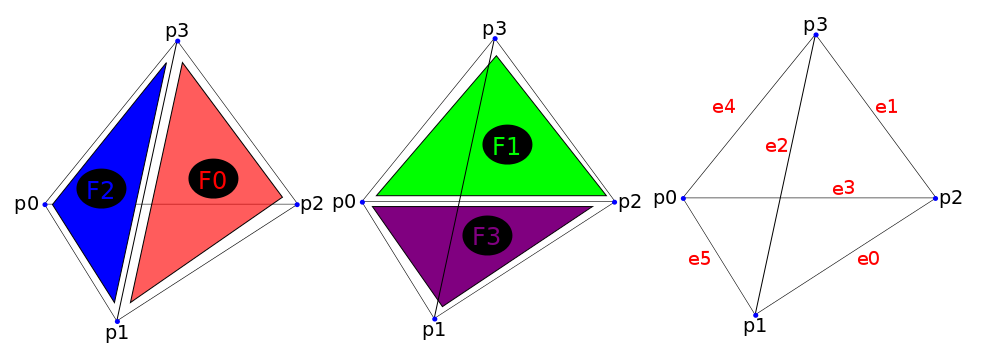
\includegraphics[width=1.0\linewidth]{figures/cutting/tetconfig3.png}
  \caption{\label{fig:tetconfig3}
  {A tetrahedral element in its canonical view. Iterating over nodes, edges and faces of each element is
  one of the primary operations in a geometric algorithm that manipulates such elements. The order we chose here is not the
  only possible one but it simplifies the cutting algorithm and element subdivision process as we will see later.}
}
\end{figure}


In a complex mesh of tetrahedral elements accessing each of these components is a necessary requirement for 
implementing any topological modifications. Therefore the main module in our cutting algorithm is an edge-based
data structure that maps tetrahedral elements to their associated faces and the faces to their associated edges and
finally the edges to their nodes. 

The minimal set of operations frequently used by most algorithms are as following \cite{Mario2010PolygonMesh}:

\begin{itemize}
 \item Access to individual vertices, edges, faces and tetrahedral elements. This includes the enumeration of 
 all elements in unspecified order.
 
 \item Access to the so-called one-ring neighborhood of the nodes. A typical use-case for this operation is the uniform 
 distribution of the external forces applied to the mesh. Also many mesh simplification algorithms predicate on such operators.
 
 \item Top-down and bottom-up hierarchical access to the mesh entities. Top-down access is inherently provided in the structure of the
 mesh entities e.g. elements are comprised of faces and faces are made up of set of edges etc. In case of the bottom up access some algorithms 
 will benefit to have the incident edges of a certain node, or in case of edges all the incident faces of a given edge and for a given face
 all the incident elements to a particular face in the mesh. This type of access patterns are particularly useful for topological modification 
 scenarios and the required book-keeping operations.
 
 \item Insertion and removal operations for nodes, edges, faces and elements. These operations require extra care in order to keep
 the top-down and bottom-up links up-to-date. As we will see in our cutting algorithm deferred removal operations can make matters alot simpler by
 delaying the actual removal until after all the identified entities are being visited and the new entities inserted to the structure.
 This is due to the fact that removal operations will update the internal links between mesh entities therefore two consecutive access operations
 might find the mesh at different states which is not intended in the original proposed algorithm.
 
 \item Update operations for nodes, edges, faces and elements. What is important here is to keep the top-down and bottom-up links up-to-date. 
 For-instance in case of an edge update as soon as the two endpoints of the edge is modified all the incident faces (higher level entity) 
 of that edge and also all the incident edges of the end points of the edge (lower level entity) should be updated.
\end{itemize}

Per each node we also store the rest position of it, this is used to update the physics model and to interpolate the position 
of newly added nodes in case of cutting. Accessing edges using the bottom-up structure is expensive: First the list of incident 
edges to one of the endpoints of the edge is accessed and then a serial search on that list is done to find an edge with the matching 
end points. This has logarithmic complexity with respect to the number of edges in the structure. Instead we chose to use a hash-table
to access edges using a key derived from the two end-points of the edge. Below is how this key is computed for a given edge:

\begin{equation}
 key64 = (nodes\left[ 1 \right] << 32) \And nodes\left[ 0 \right]
\end{equation}

This computation is performed when a new edge in inserted into the structure and can produce keys for $2^{64}$ edges uniquely. 
The hash-map then associates this key to its corresponding edge index thereby providing constant-time access. 
Using this technique the faces can also be accessed though their associated node indices which can be convenient for some applications. 

In the case of triangle faces in our tetrahedral volume mesh. After finding the edge indices for all the three edges of the given 
face using the described method above, the sublist containing the incident faces of the first edge is fetched. Using a linear search 
in that sublist the queried face can be identified. 

Nothing is removed directly from the our mesh storage buffers but rather upon cutting the elements
are marked as to\_be\_deleted and later the garbage collection removes all unreferenced items from the mesh storage buffers. 

When cutting an edge, an edge-update process is performed followed by a new edge insertion. 
The update process basically splits the original edge in two. Algorithm \ref{alg:edgesplit} describes this process
in detail which is also depicted in figure \ref{fig:splitedge}:

\begin{algorithm}[H]
\caption{Splitting an edge in our volumetric mesh data structure. The input to this algorithm is the index of the edge to be splitted
and the distance $t$ along the edge where the intersection happens. Figure \ref{fig:splitedge} shows this operation in detail. }
\label{alg:edgesplit}
\begin{algorithmic}[1]	
  \STATE $edge \gets fetchEdge(index)$
  \STATE $n0 \gets fetchNode(edge.from)$
  \STATE $n1 \gets fetchNode(edge.to)$
  \STATE $newp0.rest = n0.rest + (n1.rest - n0.rest) * t$
  \STATE $newp0.pos = n0.pos + (n1.pos - n0.pos) * t$
  \STATE $idxNewP0 \gets addNewPoint(newp0)$
  \STATE $newp1 \gets newp0$
  \STATE $idxNewP1 \gets addNewPoint(newp1)$
  
  \STATE $setEdge(index, edge.from, idxNewP0)$
  \STATE $insertEdge(idxNewP1, edge.to)$

\end{algorithmic}
\end{algorithm}



\begin{figure}[H]
  \centering
  % the following command controls the width of the embedded PS file
  % (relative to the width of the current column)
  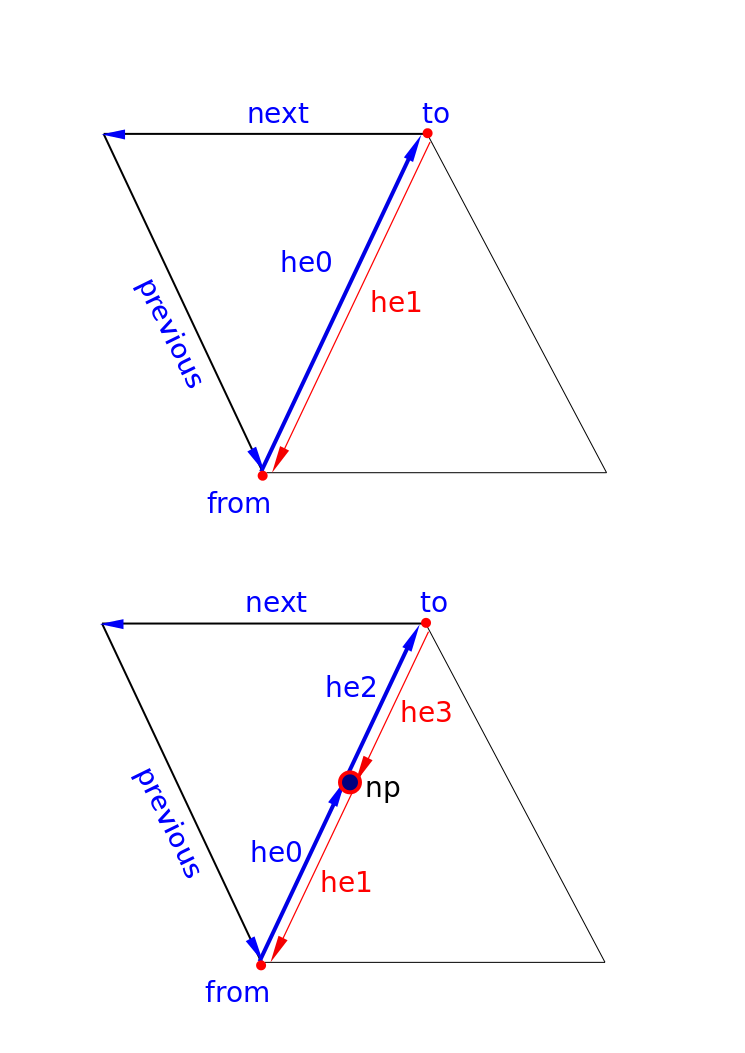
\includegraphics[width=0.8\linewidth]{figures/cutting/splitedge.png}
  \caption{\label{fig:splitedge}
  {Left: The edge to be splitted before the splitting operation described in algorithm \ref{alg:edgesplit}. 
  Right: Splitting an edge produces a new edge from the point of intersection to the original endpoint. New points $np_0$ and $np_1$ are
  initially co-located.}
}
\end{figure}


Iterating over the one-ring neighborhood nodes to a given node is performed using the following algorithm \ref{alg:oneRingNbors}:

\begin{algorithm}[H]
\caption{Iterating over one-ring neighborhood nodes of a given node.}
\label{alg:oneRingNbors}
\begin{algorithmic}[1]	
  \STATE $incidentEdges \gets incident_edges_to_node(node)$
  
  \FOR{$i = 0$ \TO $incidentEdges.count - 1$} 
  \STATE $edge \gets incidentEdges\left[i\right]$
  \IF{$edge.from \neq node$}
  \STATE $nbors.insert(edge.from)$
  \ELSE
  \STATE $nbors.insert(edge.to)$
  \ENDIF
  \ENDFOR
  \RETURN $nbors$
\end{algorithmic}
\end{algorithm}

Upon topological modification, events are generated to notify cutting algorithms of the internal changes in the mesh structure. 
This is also useful for debugging and evaluation purposes and can be logged for accounting the sequence of changes made to the 
original mesh. The events include update, insertion and removal of nodes, edges, faces and elements.


In the next section we describe the cutting algorithm which is based on the edge-based data structure presented in this section.

\section{Cutting Algorithm}
Our cutting algorithm follows the same strategy presented by Ganovelli \etal \cite{Ganovelli2000} which suggests use of lookup tables to 
handle different configurations. We also applied the optimizations suggested by
Steinemann and Mor \etal \cite{Steinemann, Mor2000} to have minimal new elements added to the mesh under cut. 
The first stage in our cutting algorithm is detecting the cut sweep-surface. The input to this stage is the cut trajectory which is a list of points
that the scalpel passed through in Euclidean space. The cut trajectory is not collected until the axis-aligned bounding box of the cutting tool intersects
with that of the tissue. The tissue bounding box is expanded to rule out the boundary cases where the surface of the model contacts with its own bounding 
box. In such cases the scalpel might miss the surface if the bounding box test fails to detect the initial contact. 

\begin{figure}[H]
  \centering
  % the following command controls the width of the embedded PS file
  % (relative to the width of the current column)
  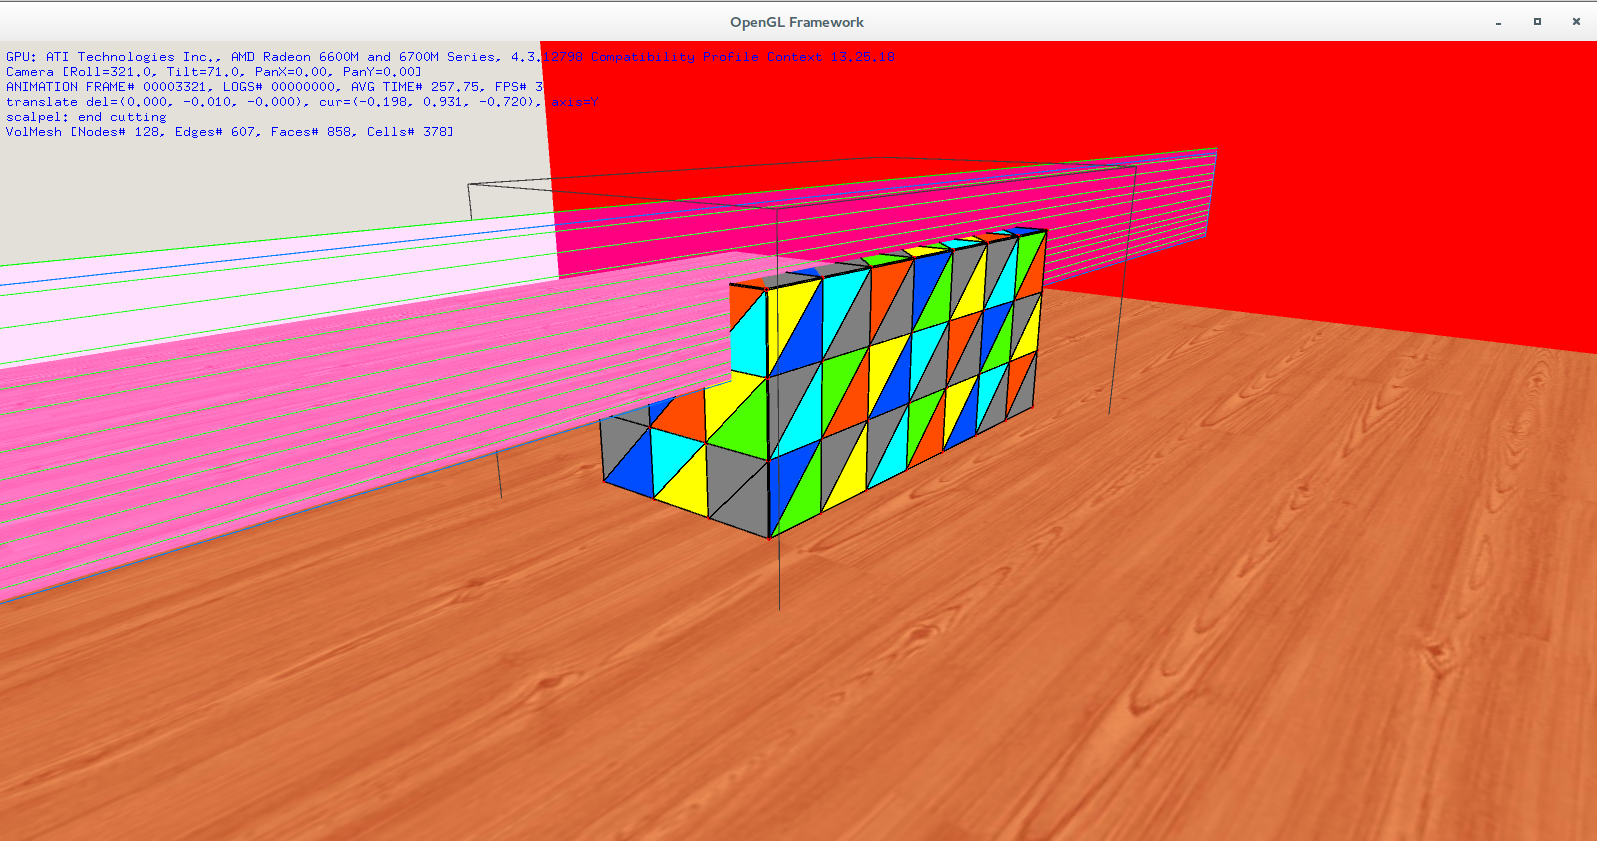
\includegraphics[width=0.6\linewidth]{figures/cutting/cubecut02.png}
  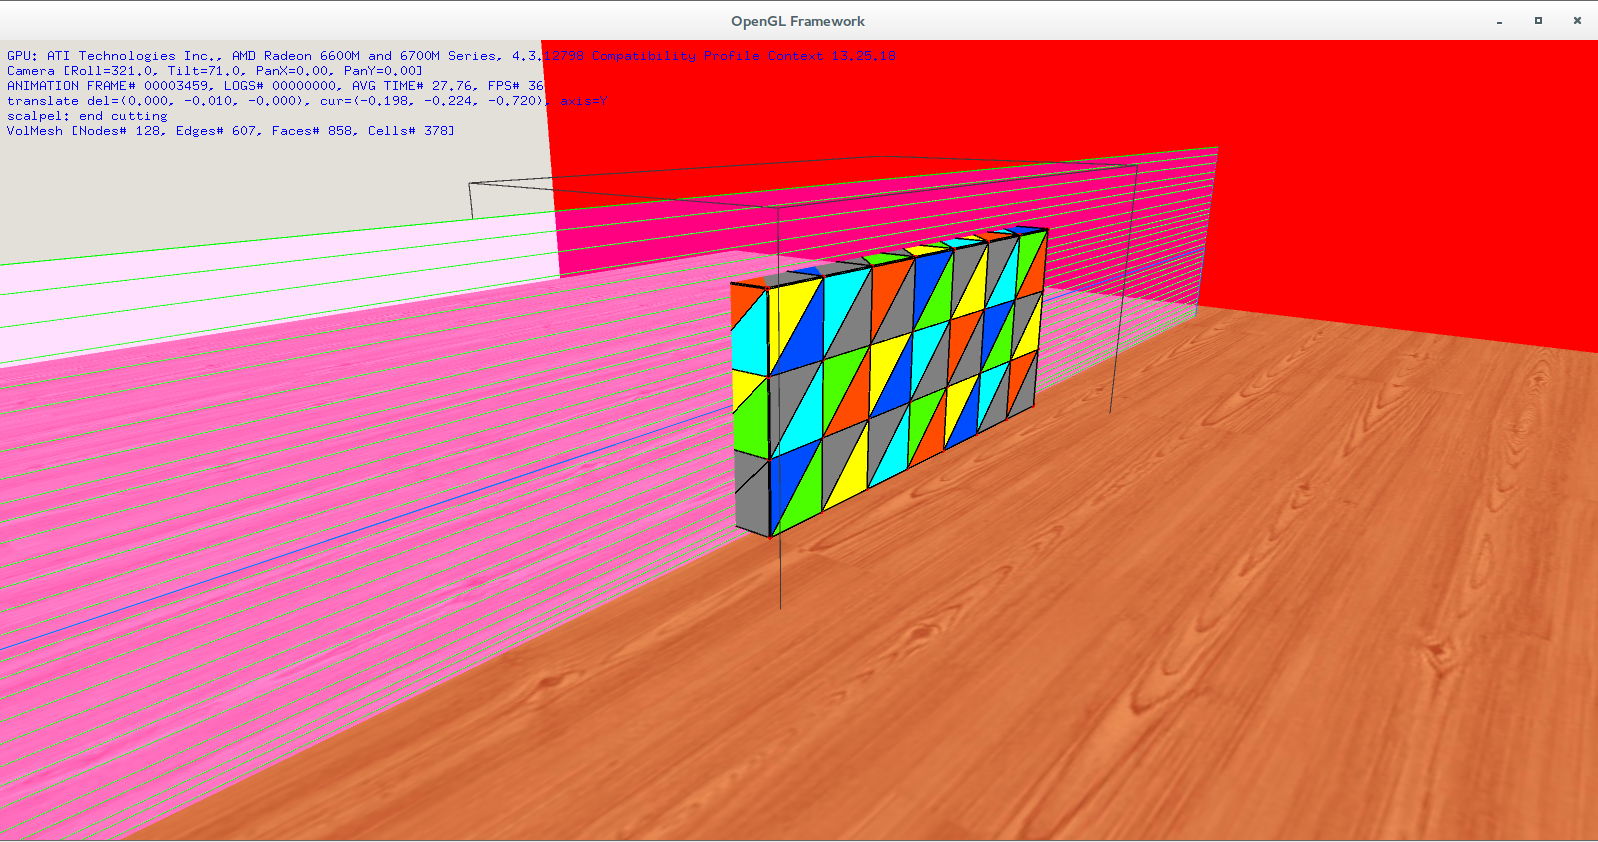
\includegraphics[width=0.6\linewidth]{figures/cutting/cubecut04.png}
  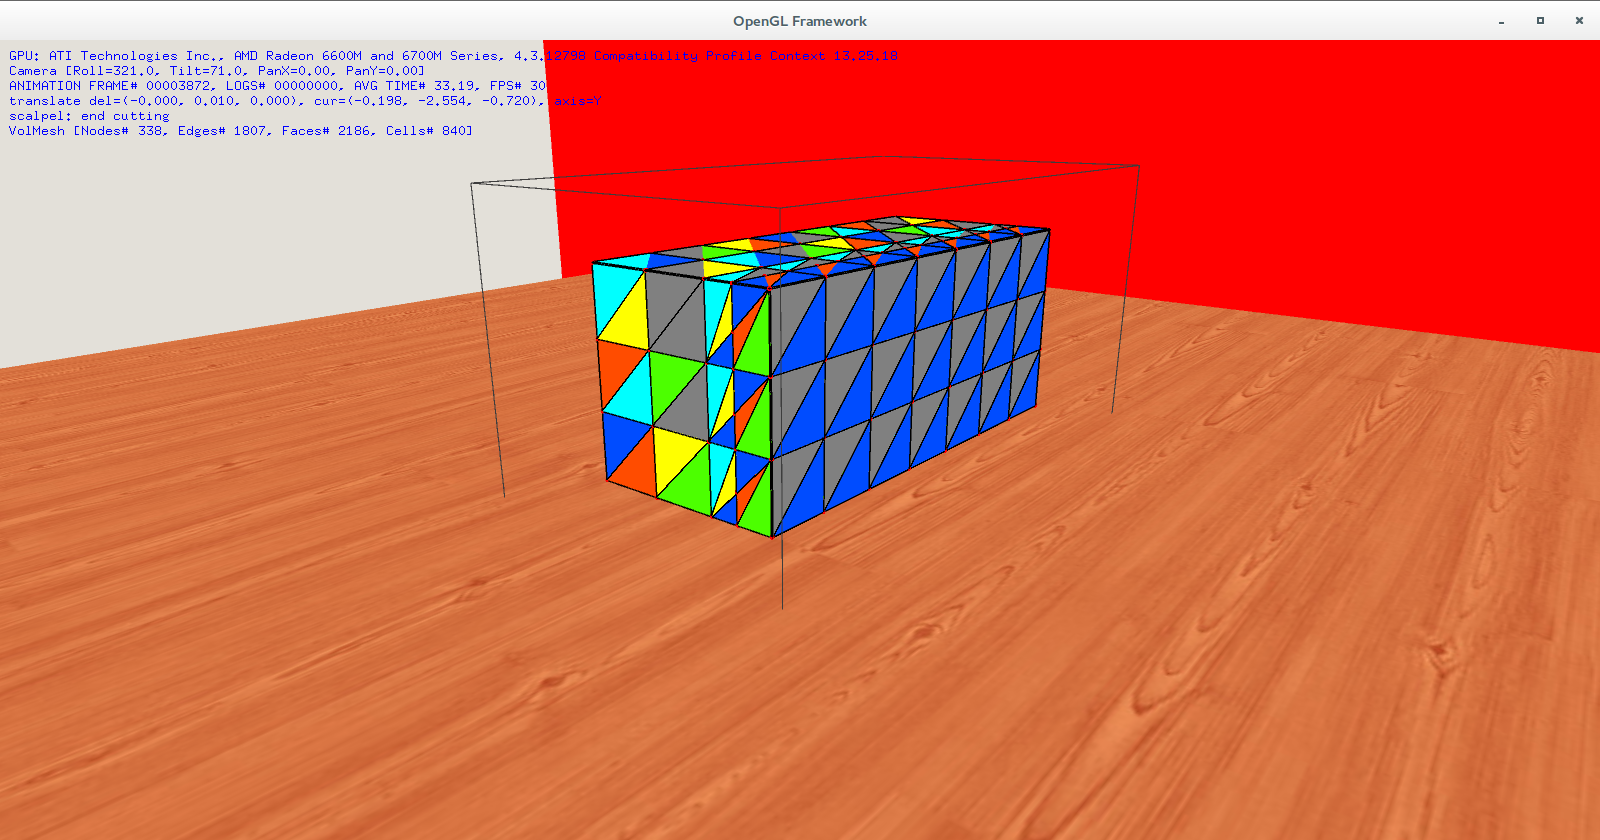
\includegraphics[width=0.6\linewidth]{figures/cutting/cubecut05.png}

  \caption{\label{fig:sweepsurf}
  {The cut trajectory in blue and the sweep-surface shown in pink. The scalpel passes through the voxel grid model for cutting.}
}
\end{figure}

\subsection{Edge Intersections}
Using a GPU kernel function the intersection of the sweep-surface and all the edges of the model are computed. 
The input to this stage is the list of edges of the model and 4 points defining the sweep-surface quadrilateral. 
Since the intersection of a triangle and a line segment is faster to compute than a quadrilateral, we 
use two intersection tests per each edge to figure out wether the segment is splitted or not. The implementation
of our edge triangle intersection follows the Ray-Triangle intersection test given in \cite{RTR3}.


Similar to our GPU polygonization method in section \ref{sec:surfextraction}, a prefix-sum operator counts the number
of intersections and also compacts the resulting array of intersection points. The final output of this stage is a list
of intersection points and the associated edge indices. Listing below shows the prototype of the kernel function in 
OpenCL:

\begin{lstlisting}[frame=single]
//Computes the intersection of edges and sweepsurface
float sweepSurfEdgeIntersections(unsigned int countEdges,
			         __global float4* edgeBuffer,
				 __global float4 sweepSurface[4],
				 __global float4* scanIntersections,
				 __global unsigned int* scanIndices,
				 __global unsigned int* scanFlags);
\end{lstlisting}
		     
\begin{algorithm}[H]
\caption{\textit{EdgeIntersections} The kernel function that computes intersections of edges 
and the sweep-surface. The prototype of the kernel follows the listing above and the algorithm here represents one 
thread of the execution. }
\label{alg:edgeIntersections}
\begin{algorithmic}[1]	
  \IF{$dim.x \geq countEdges$}
  \STATE return
  \ENDIF
  \STATE $scanFlags[dim.x] \gets 0$
  \STATE $tri0 \gets triangle(0, 1, 2, sweepSurface)$
  \STATE $tri1 \gets triangle(0, 2, 3, sweepSurface)$
  \STATE $edge0 \gets edgeBuffer[dim.x * 2]$
  \STATE $edge1 \gets edgeBuffer[dim.x * 2 + 1]$
  \STATE $res \gets IntersectSegmentTri(edge0, edge1, tri0, p)$
  \IF{$res = 0$}
  \STATE $res = IntersectSegmentTri(edge0, edge1, tri1, p)$
  \ENDIF
  \IF{$res \neq 0$}
  \STATE $scanIntersections[dim.x] \gets p$
  \STATE $scanIndices[dim.x] \gets dim.x$
  \STATE $scanFlags[dim.x] \gets 1$
  \ENDIF
  
\end{algorithmic}
\end{algorithm}


%The main contribution of our cutting method is the GPU-accelerations applied to the cutting process to support interactive topological 
%modifications and the post processing step that supports smoothness of the cuts in case of complex tissues. 

